\documentclass[11pt, english]{article}

\usepackage{graphicx}
\usepackage[colorlinks=true, linkcolor=blue]{hyperref}
\usepackage[english]{babel}
%\selectlanguage{english}
\usepackage[utf8]{inputenc}
\usepackage[svgnames]{xcolor}
\usepackage{amsmath}
\usepackage{enumitem}
\usepackage{multicol}
\usepackage{enumitem}

\usepackage{listings}
\usepackage{afterpage}

\usepackage{float}
\restylefloat{table}

\pagestyle{plain}

\definecolor{dkgreen}{rgb}{0,0.6,0}
\definecolor{gray}{rgb}{0.5,0.5,0.5}
\definecolor{mauve}{rgb}{0.58,0,0.82}

%\lstset{language=Python,
%    basicstyle=\small\ttfamily,
%   stringstyle=\color{DarkGreen},
%    otherkeywords={0,1,2,3,4,5,6,7,8,9},
%    morekeywords={TRUE,FALSE},
%    deletekeywords={data,frame,length,as,character},
%    keywordstyle=\color{blue},
%    commentstyle=\color{DarkGreen},
%}

\lstset{frame=tb,
language=R,
aboveskip=3mm,
belowskip=3mm,
showstringspaces=false,
columns=flexible,
numbers=none,
keywordstyle=\color{blue},
numberstyle=\tiny\color{gray},
commentstyle=\color{dkgreen},
stringstyle=\color{mauve},
breaklines=true,
breakatwhitespace=true,
tabsize=3
}


\textheight=21cm
\textwidth=17cm
%\topmargin=-1cm
\oddsidemargin=0cm
\parindent=0mm
\pagestyle{plain}

\usepackage{color}
\usepackage{ragged2e}

\global\let\date\relax
\newcounter{unomenos}
\setcounter{unomenos}{\number\year}
\addtocounter{unomenos}{-1}
\stepcounter{unomenos}
\gdef\@date{ Course \arabic{unomenos}/ 2019}

\begin{document}


\begin{titlepage}

\begin{center}
\vspace*{-1in}
\begin{figure}[htb]
\begin{center}

\includegraphics[width=5cm]{Resources/BicoccaLogo.png}
%\hspace{\fill} %Space between images
%\includegraphics[width=3cm]{sea-vision-official-logo.png}
\end{center}
\end{figure}
UNIVERSITÀ DEGLI STUDI MILANO - BICOCCA \\
\vspace*{0.4in}
\begin{large}
Information Retrieval Project Exam\\
\end{large}
\vspace*{0.2in}
\begin{Large}
\textbf{IRPersonalNews Project} \\
\vspace*{0.15in}
Information Retrieval Personalized News System \\
\end{Large}
\vspace*{0.3in}

\vspace*{0.3in}
\rule{80mm}{0.1mm}\\
\vspace*{0.1in}
\begin{large}
Andrea Guzzo - 761818
\end{large}
%\includegraphics[width=8cm]{yudoo-image.jpg}
\end{center}
\end{titlepage}

\newcommand{\CC}{C\nolinebreak\hspace{-.05em}\raisebox{.4ex}{\tiny\bf +}\nolinebreak\hspace{-.10em}\raisebox{.4ex}{\tiny\bf +}}
\def\CC{{C\nolinebreak[4]\hspace{-.05em}\raisebox{.4ex}{\tiny\bf ++}}}

\tableofcontents
\newpage
\section{Introduction}

In the Web 2.0 era one of the most important and relevant aspects is to try to organize, filter and select news and information in a way that is more relevant to our interests, our purpose and our goal. 
\newline
This result can be achieved thanks to recommendation engines that allow to select, filter and propose to the user only a series of relevant contents and information in order to be able to unravel more effectively in the digital jungle of constant content. 
\newline
This aspect of dynamism and speed of information is particularly relevant in the world of social networks.
\newline \break
This project therefore proposes an automatic system that allows the user to filter messages on twitter based on several factors: words written by the user, some reference topics and articles previously read by the user himself in order to provide different levels of customization of the information.
\newline \break
The project is part of the Information Retrieval master degree exam at Università degli Studi Milano-Bicocca.
The implementation follow the project requirement specification A: A personalized search engine for microblog contents.

\newpage

\section{Proposed Solution}

The system created is divided into four parts connected to each other:
\begin{enumerate}
\item News downloader and parsing
\item Tweets downloader and parsing
\item Profiles and index builder
\item Online document retrieval website
\end{enumerate}
This four parts are linked each other by a system pipeline described in the following image:

\begin{figure}[H]
  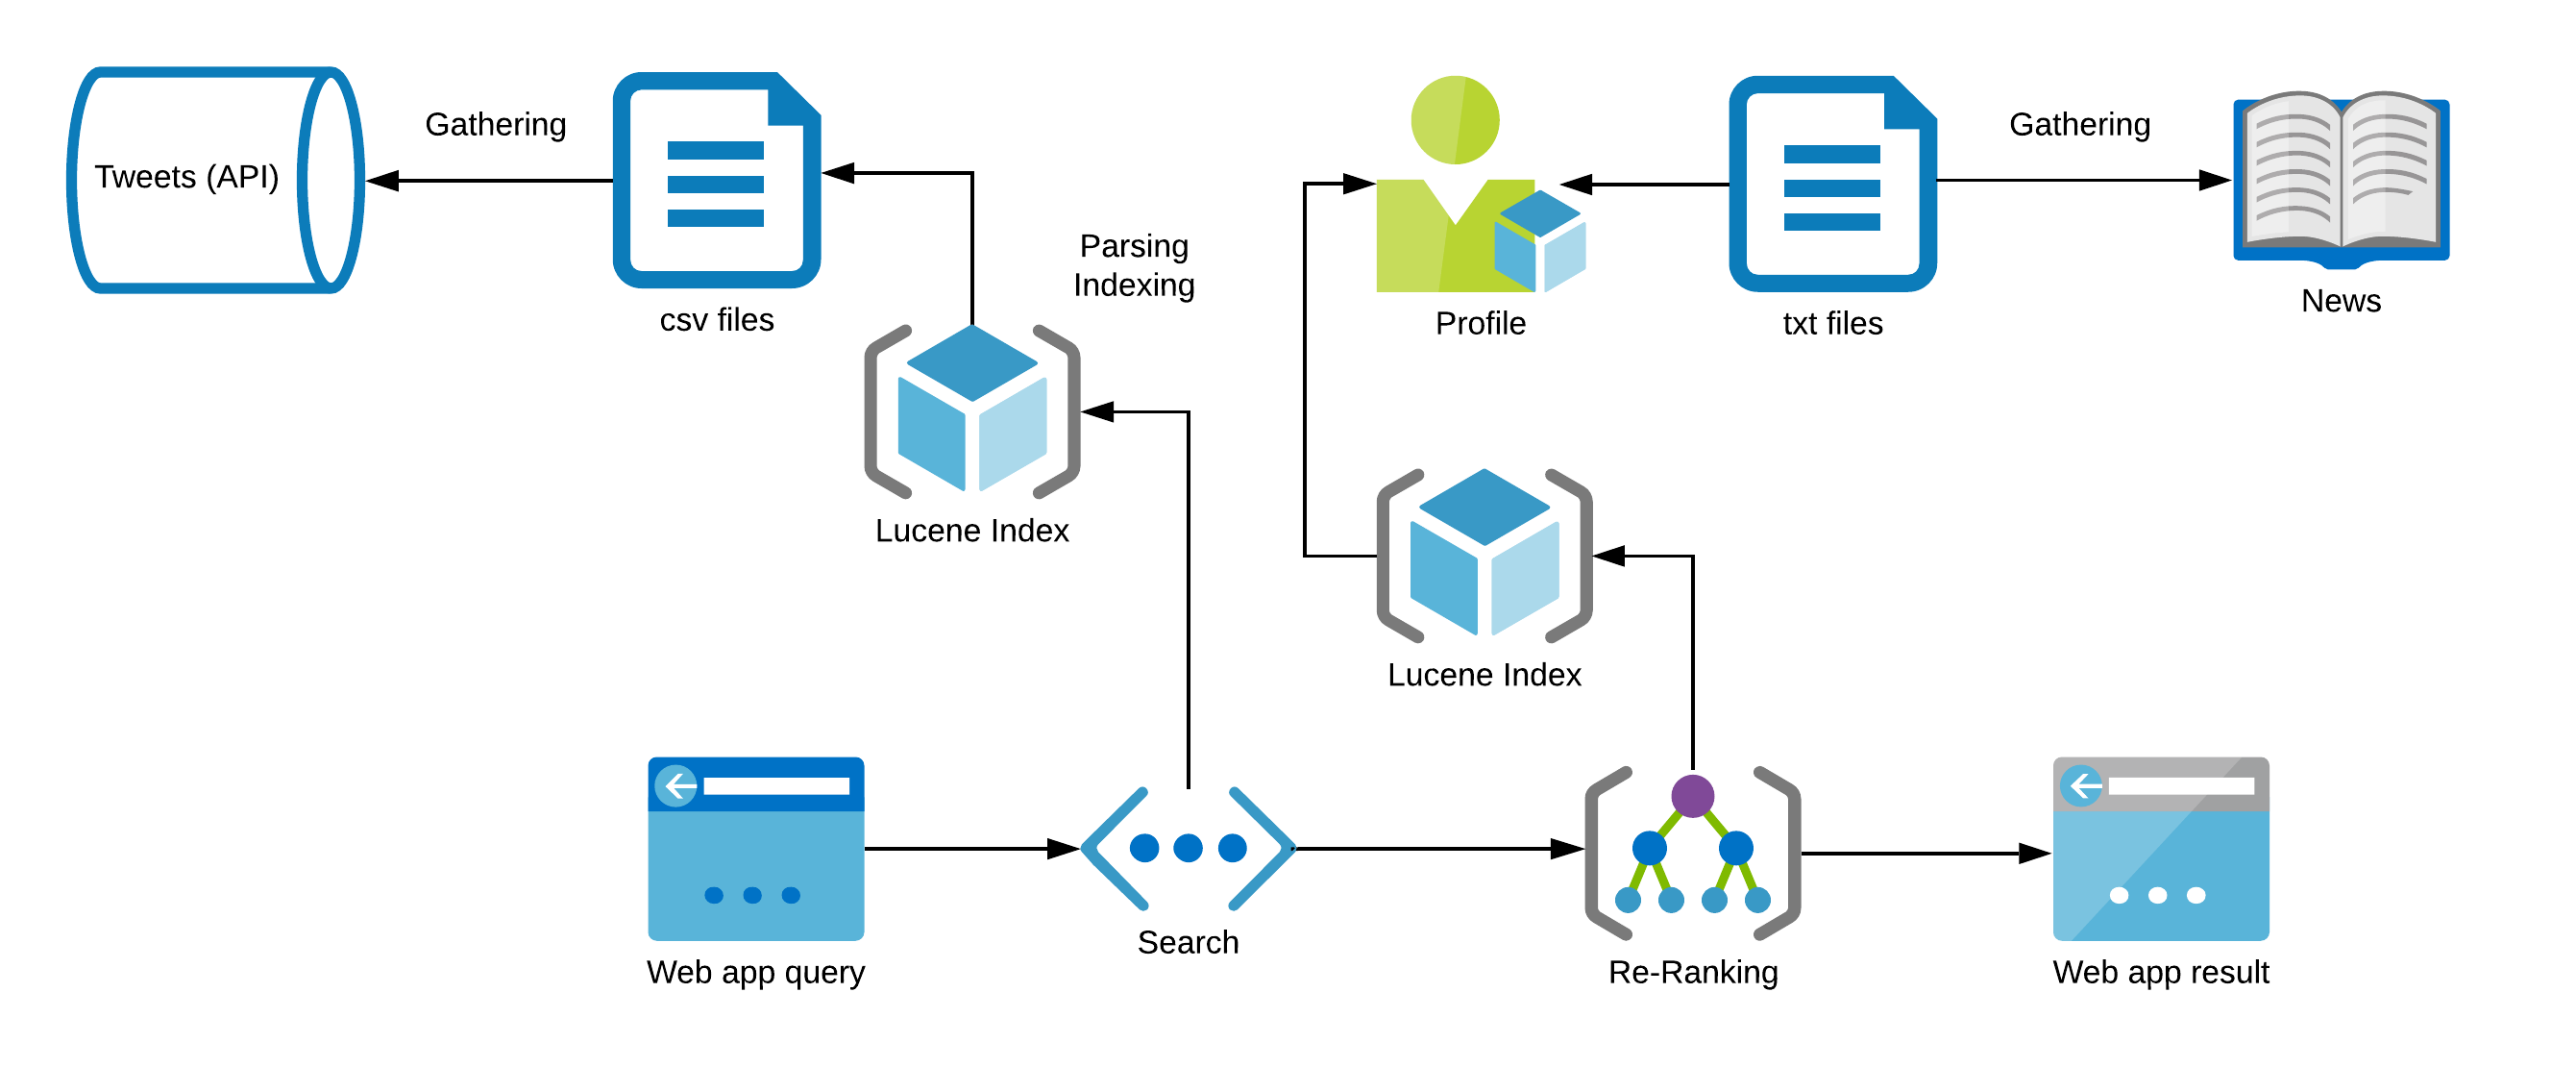
\includegraphics[width=16cm]{Resources/OverallArchitecture.png}
  \caption{News Gathering Pipeline} 
\end{figure}

The technologies used are as follows:
\begin{itemize}
\item Python with libraries: 
\item Java with Sping Framework for the front-end and backend implementation
\item Lucene: for index builder
\item Html, Css, Javascript
\end{itemize}

The first and the second parts are described into the information gathering section in this document.
The Profiles and Online document retrieval system into the IR System section.
Finally the website implementation is described in the last dedicated section.

\subsection{Information gathering}

The information gathering is divided in two different part: the news and the tweet downloading and parsing.
All the information obtained are in English language.
In order to maintain a certain consistency between the input data with respect to any user preferences and in accordance with the graphical interface and usability, it was decided to focus the collection of information on a few relevant topics:
\begin{multicols}{3}
\begin{itemize}
\item Politics
\item Tech
\item Sport
\item Life
\item Science
\end{itemize}
\end{multicols}

In the news gathering part the sites from which the data are collected are:
\begin{itemize}
\item Politics: BBC, CNN
\item Tech: Verge, Wired
\item Sport: BBC, Eurosport
\item Life: Vogue, Independent
\item Science: Scientific American, Science Mag
\end{itemize}

For every site we have obtained 5 random articles in a certain period of time, so in total we used 10 article for every topics.

\begin{figure}[H]
  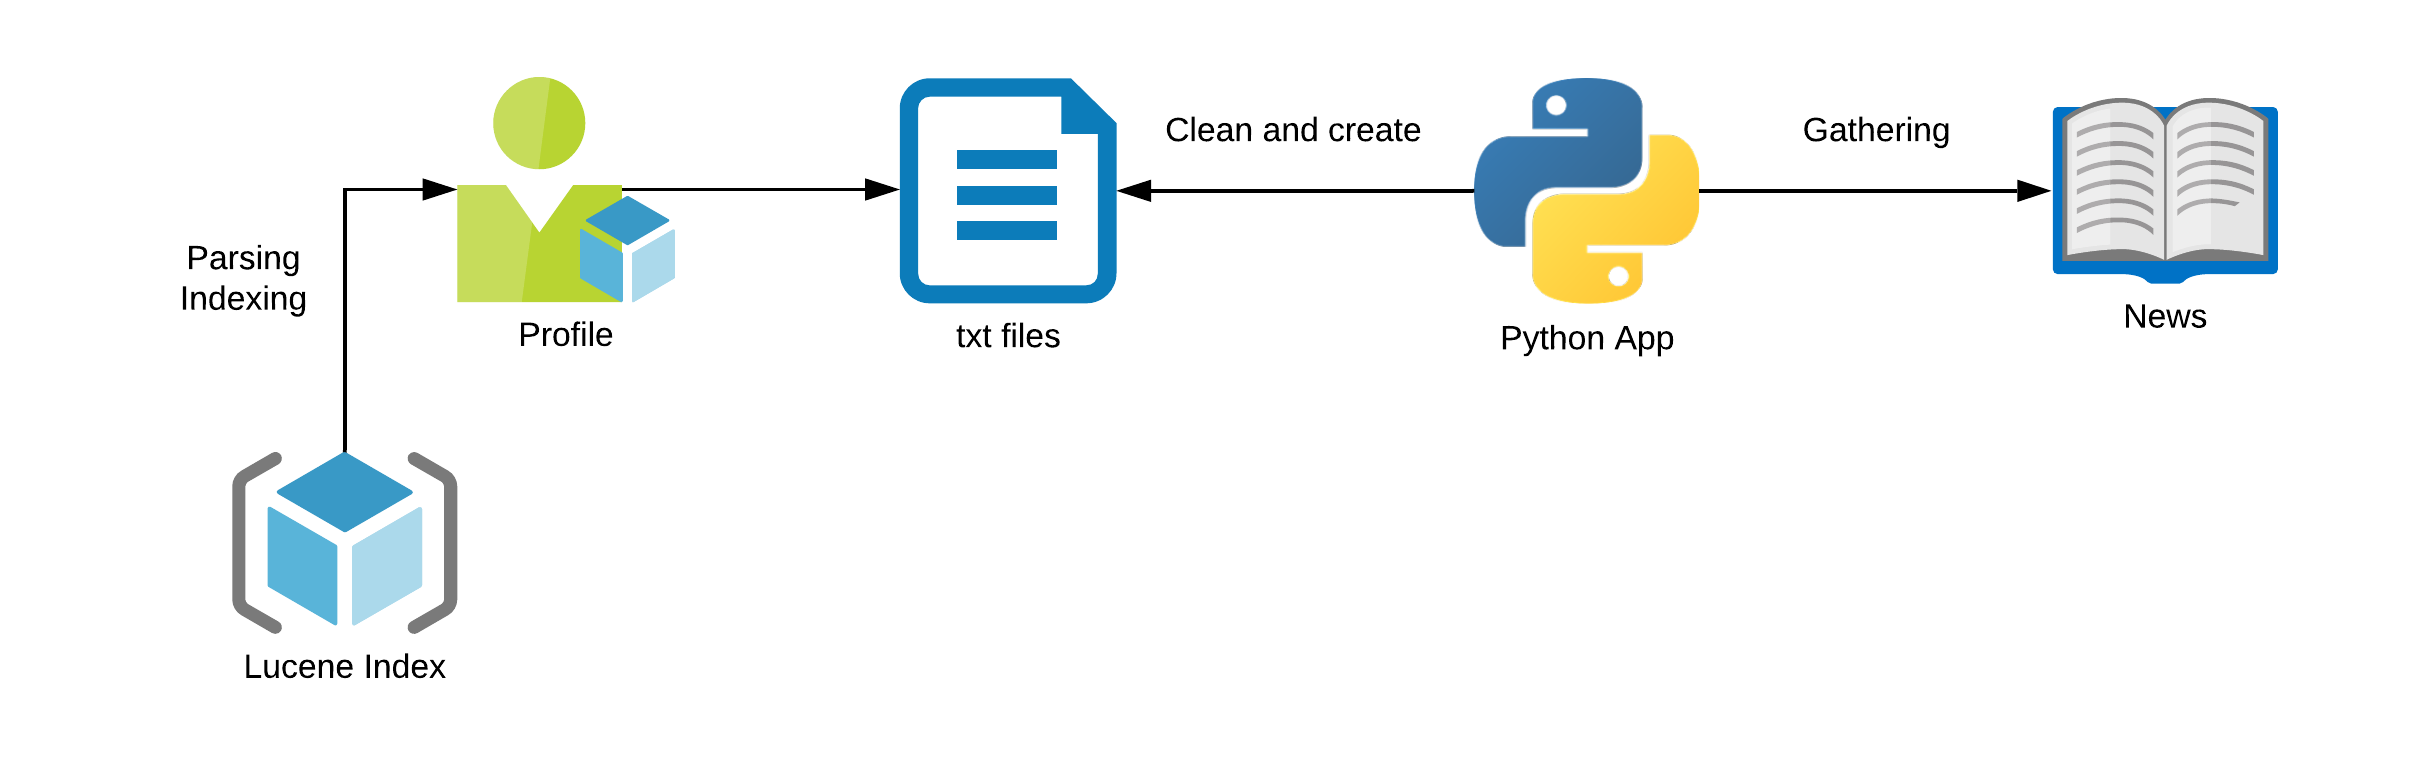
\includegraphics[width=16cm]{Resources/News.png}
  \caption{News Gathering Pipeline} 
\end{figure}


The second tweet gathering application use a query with the topic name as search criteria over a collection of profile, retrieving every information written in a month for a maximum of 3000 tweets (30.000 tweets in total), a limit due to authentication problems on the official APIs.
For the tweet gathering part the profile from which the tweet are collected are:
\begin{itemize}
\item Politics: BBCPolitics, CNNPolitics
\item Tech: Verge, WiredUk
\item Sport: BBCSport, Eurosport
\item Lifestyle: Voguemazine, IndyLife
\item Science: Sciam, Sciencemagazine
\end{itemize}

\begin{figure}[H]
  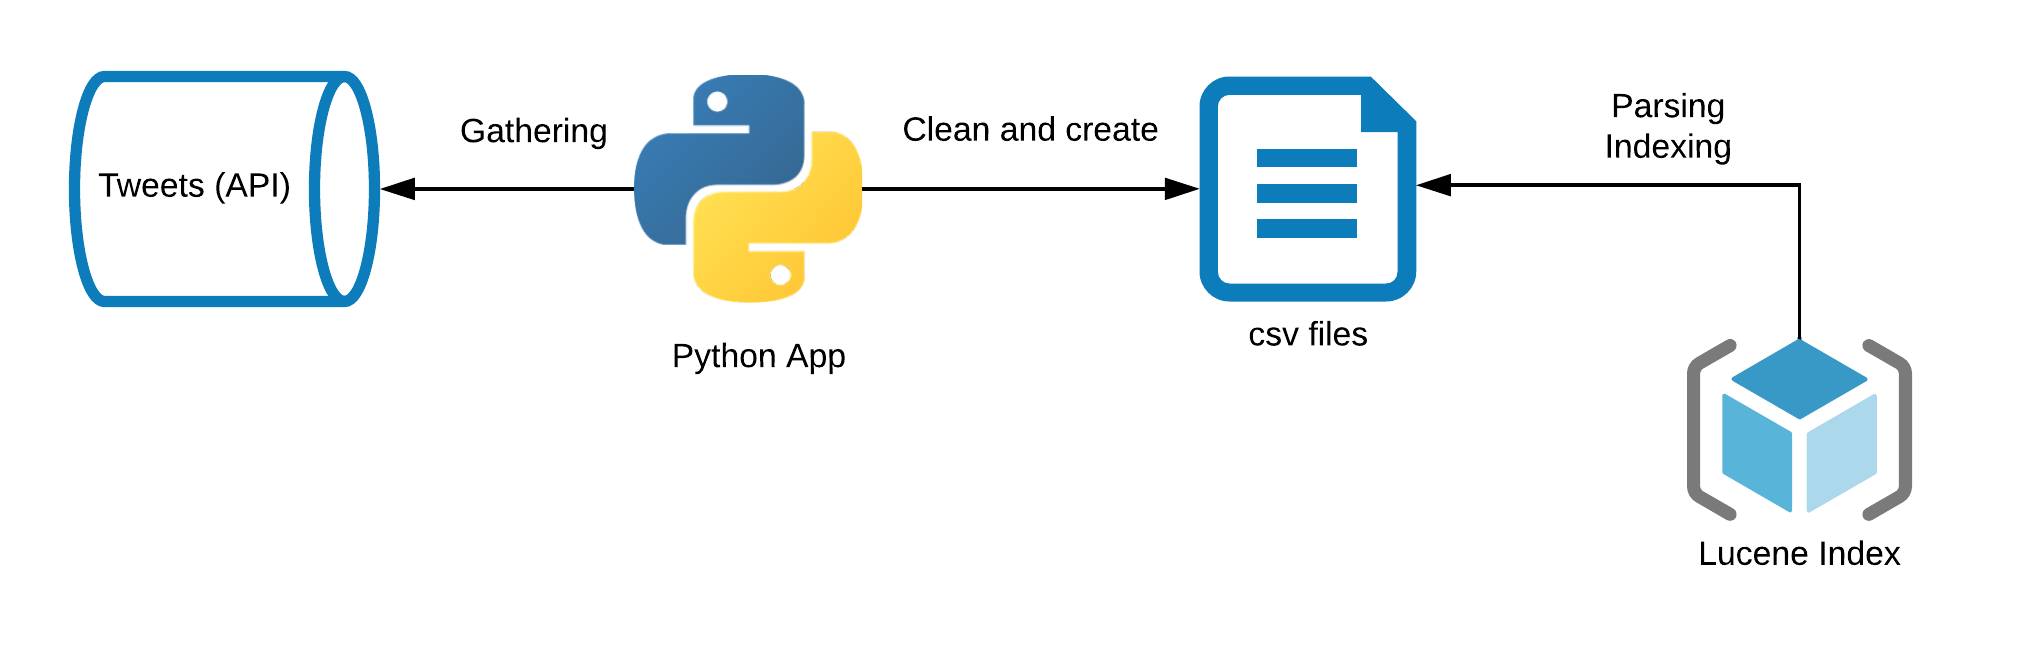
\includegraphics[width=16cm]{Resources/Tweets.png}
  \caption{News Gathering Pipeline} 
\end{figure}

The tweets downloaded contains this following information:
\begin{multicols}{3}
\begin{itemize}
\item Tweet ID
\item Permalink
\item Username
\item Text
\item Date
\item Retweet
\item Favorite
\item Mentions
\item Hashtag
\item Geo-info
\end{itemize}
\end{multicols}

All this Information Gathering part are written in Python and use this libraries:
\begin{itemize}
\item News: Newspaper, Pandas
\item Tweets: GetOldTweets, Pandas
\end{itemize}

A minimum parsing of the downloaded information was also performed to remove incorrect results with obvious textual anomalies (e.g.: missing data, incorrectly coded characters, aggregation of tweets, selection of useful information).



\newpage

\subsection{IR System}

The IR library used for indexing and searching the knowledge based obtained is Apache Lucene.
Lucene is a high performance, scalable Information Retrieval (IR) open source library. It lets the developers indexing and searching capabilities for an applications.
It's implemented in Java and it's a member of the populare Apache Jakart family of projects, licensed under the liberal Apache Software License.
Is currently, and has been for a few years, the most popular free Java IR Library.

One of the main advantage is that Lucene doesn't care about the source of the data, its format, or even its language, as long as you can convert it to text. This means you can use Lucene to index and search data stored in files: web pages on remote web servers, documents stored in local file systems, simple text files, Microsoft Word documents, HTML or PDF files, or any other format from which you can extract textual information.

A typical application integration architecture with Lucene is:

\begin{figure}[H]
  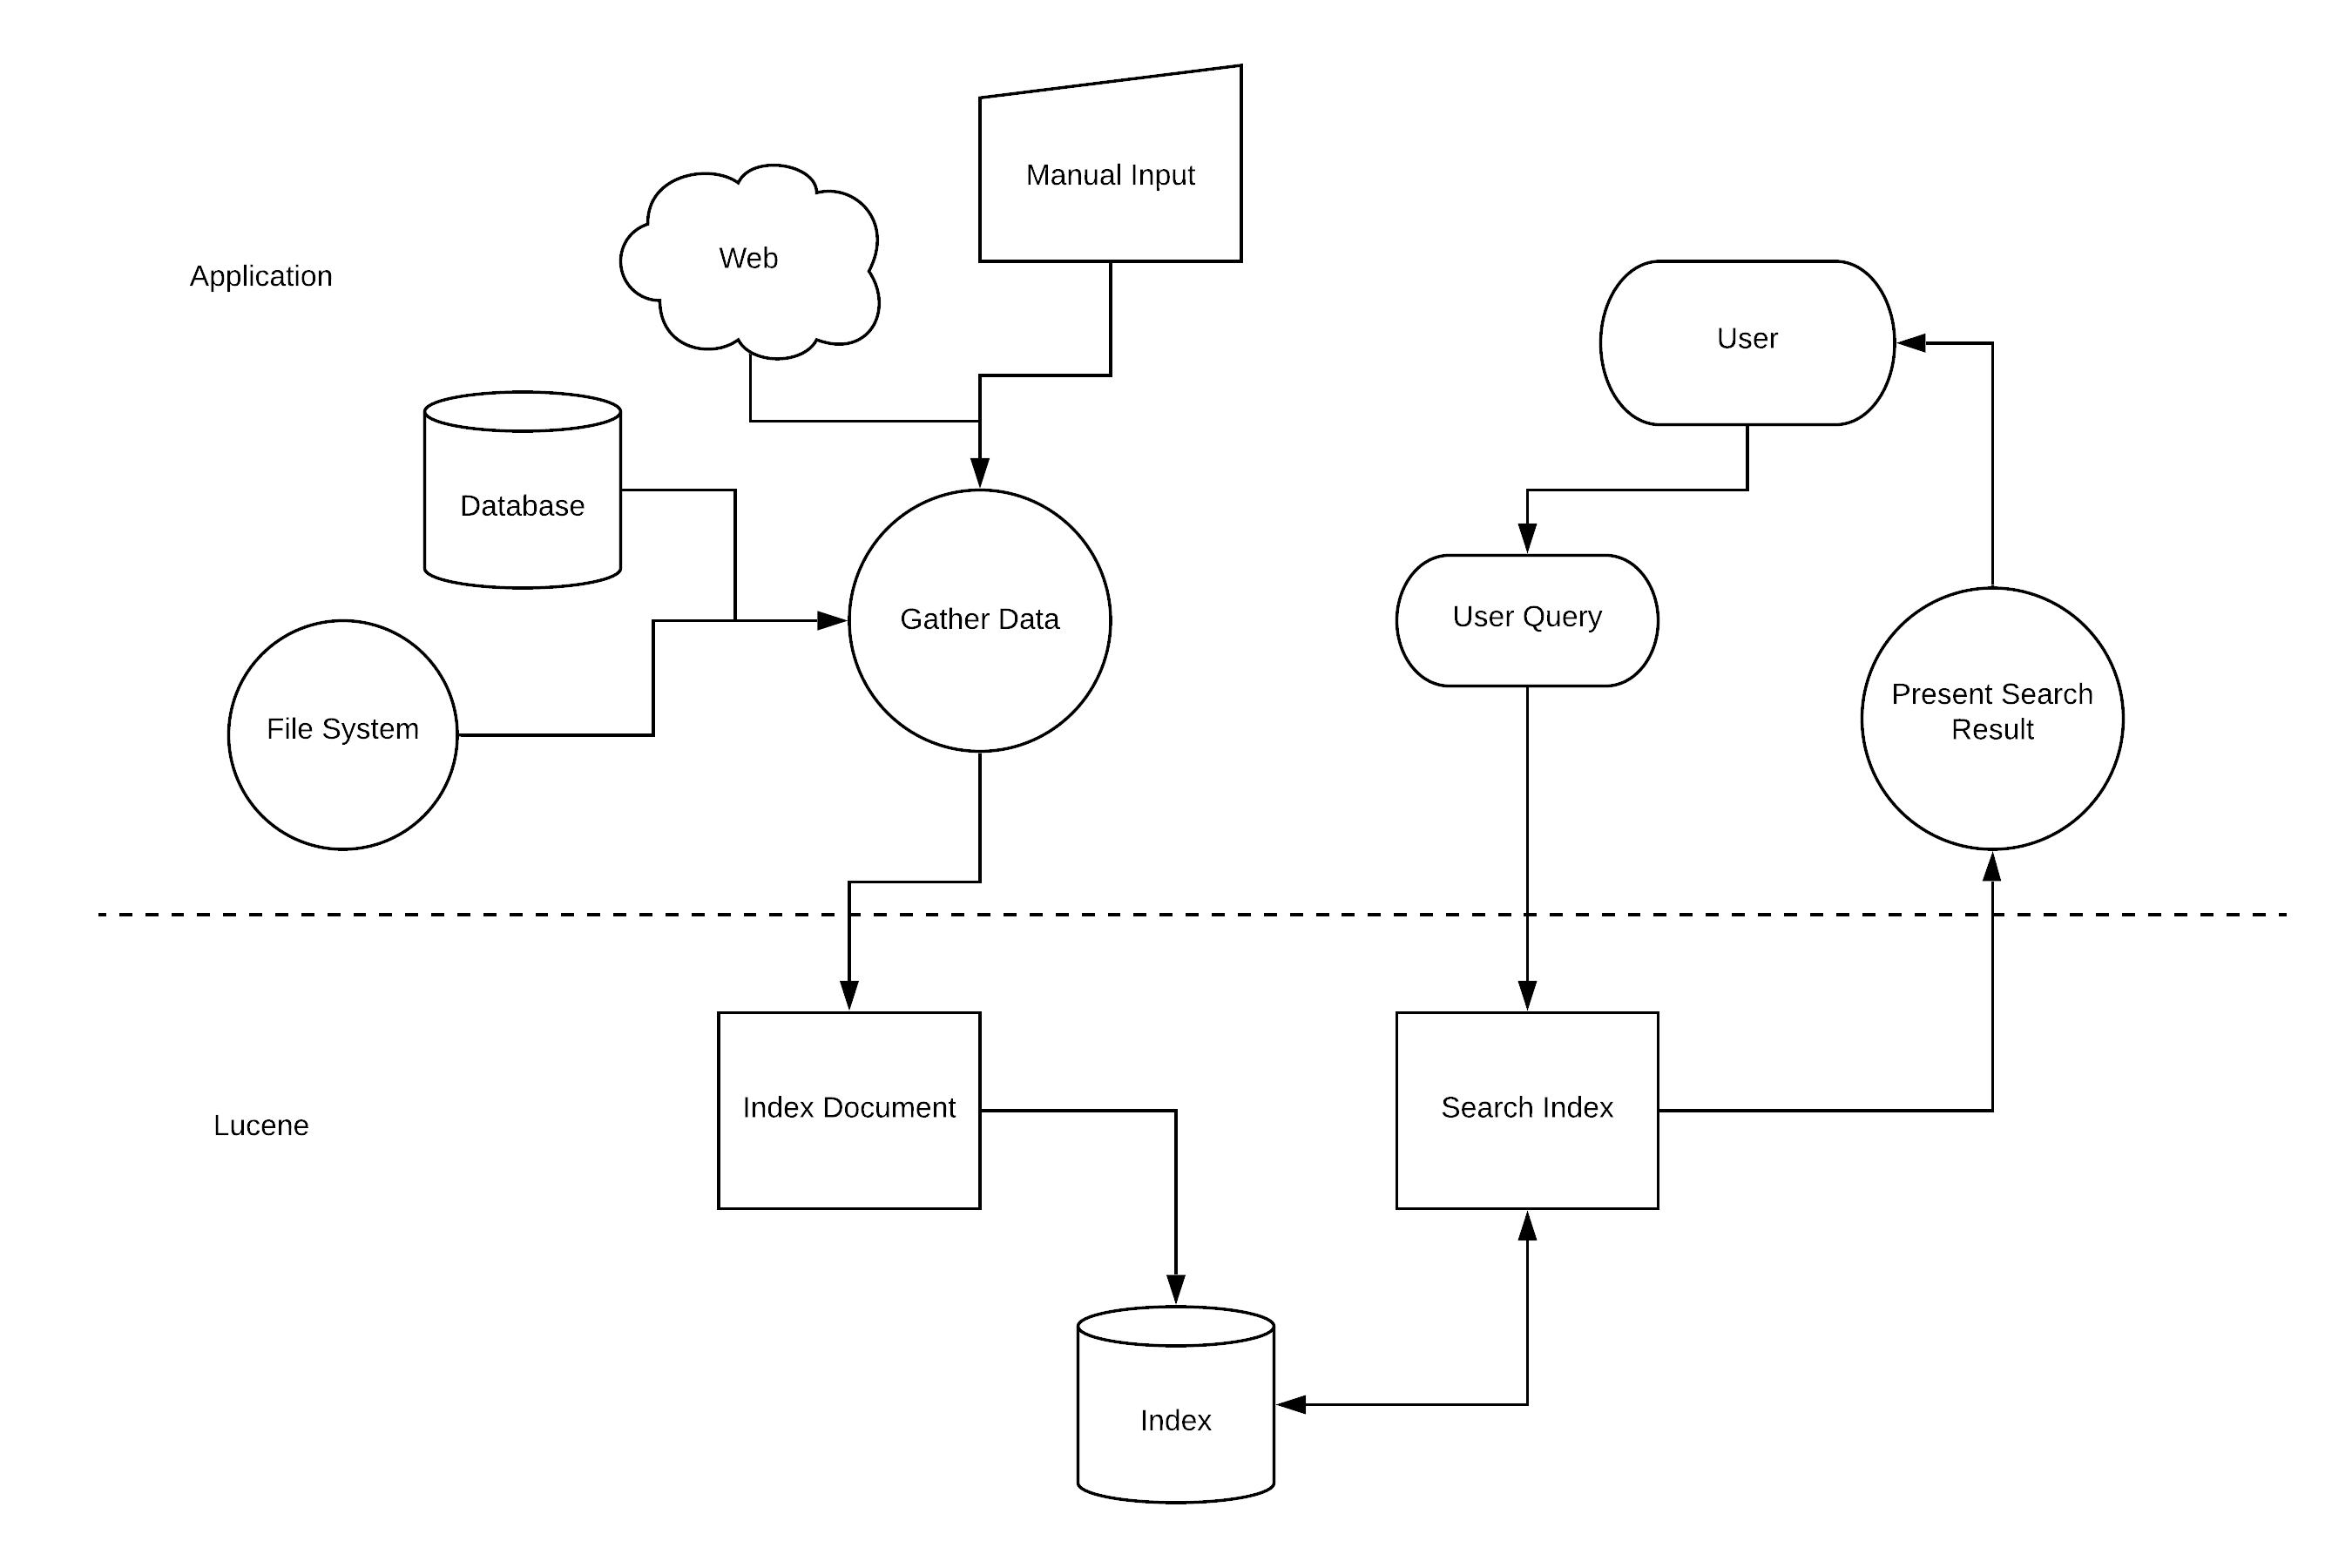
\includegraphics[width=16cm]{Resources/IRLuceneArchitecture.png}
  \caption{News Gathering Pipeline} 
\end{figure}

The architecture implemented and described in the previous chapters fits the typical definition of Information Retrieval systems as in the previous image

\subsubsection{Indexing}

The existing indexes within the solution are those generated using the latest version of the downloaded news and tweets, all other versions have been removed for consistency and project cleanliness.

To calculate the indexes it was decided to use only the text contained in the tweets and news for reasons of simplicity, we did not take into account other available information such as: hashtags, images, dates, news title, etc...

Tweet dates and number of retweets were used to build and have a performance boost on recent and most popular documents. To implement this correction mechanism, Lucene's "NumericDocValueField" was used.

The other fields remained within the index for demonstration purposes only and were easily used in a later release or testing.

For text analysis and document cleaning a "CustomAnalyzer" was used which uses a grammar-based tokenizer, a stemmer and stop words removal ignoring the case with a pre-filter on words based on regular expressions

\subsubsection{Retrieval}

The retrieval process is based on the user query and act over the tweet index generated in the preprocessing pipeline.
The retrieval model used in the system in Okapi BM25 that improves upon TF*IDF. 
\break
BM25 stands for “Best Match 25”. Released in 1994, it’s the 25th iteration of tweaking the relevance computation. BM25 has its roots in probabilistic information retrieval. Probabilistic information retrieval casts relevance as a probability problem. A relevance score, according to probabilistic information retrieval, ought to reflect the probability a user will consider the result relevant.
\break
Here it's an \hyperlink{https://opensourceconnections.com/blog/2015/10/16/bm25-the-next-generation-of-lucene-relevation/}{explanation} why this metric it's important instead using the classic TF*IDF implementation
\newline
The probabilistic information retrieval problems are well described in this \hyperlink{https://nlp.stanford.edu/IR-book/html/htmledition/probabilistic-information-retrieval-1.html}{document} of NLP Stanford departemente and course.
\newline

Given a query Q and a document D, the BM25 is defined as:
\begin{equation}
score(D, Q) = \sum_{i=1}^{n} IDF(q_i) \cdot \frac{f(q_i, D)\cdot(k_i + 1)}{f(q_i, D) + k_1 \cdot \bigg(1 - b + b \cdot \frac{|D|}{avgdl}\bigg)}
\end{equation}
\begin{equation}
IDF(q_i) = \log \frac{N - n(q_i) + 0.5}{n(q_i) + 0.5}
\end{equation}
Where:

\begin{itemize}[noitemsep]
\item $f(q_i, D)$ is $q_i$'s term frequency in the document $D$;
\item $|D|$ is the length of document $D$;
\item $avgdl$ is the average document length in the collection;
\item $k_1$ and $b$ are free parameters, with optimal values $k_1 \in [1.2, 2.0]$ and $b=0.75$;
\item $N$ is the number of documents in the collection;
\item $n(q_i)$  is the number of documents containing $q_i$. 
\end{itemize}

\subsection{Personalization}

In order to achieve the goal of creating a news search system starting from twitter posts and customized according to the user's preferences (how many and which articles he read on which topic), it was necessary to implement a customization phase of the results according to the user's interests.

In this section will be presented the customization of the results according to the user and the analytical approach used to generate the preferences.

\subsubsection{User Custom Profiles}

The construction of user profiles uses a preference system.
A user can have 3 class of interests each related to a particular topic. Each class of interest is associated also with a different number of articles

\begin{itemize}
\item class 1: main interest: 5 random articles in a topic
\item class 2: sideshow: 3 random articles in a topic
\item class3: hobby: 1 random article in a topic
\end{itemize}

In this regard, the following table has been created to map and build user profiles in order to map classes against the topic and to insert the correct number of articles in each profile respectively

% Please add the following required packages to your document preamble:
% \usepackage{graphicx}
\begin{table}[H]
\centering
\resizebox{\textwidth}{!}{%
\begin{tabular}{l|lllll|ll}
User & Politics & Technology & Science & Sport & Lifestyle & Polarize Interest & Secondary Interest \\ \hline
1    & 1        & 2          & 3       &       &           & Politics          & Technology         \\
2    & 1        &            & 2       & 3     &           & Politics          & Science            \\
3    &          & 1          & 2       & 3     &           & Technology        & Sport              \\
4    & 3        & 1          & 2       &       &           & Technology        & Science            \\
5    & 3        & 2          & 1       &       &           & Science           & Technology         \\
6    &          &            & 1       & 2     & 3         & Science           & Sport              \\
7    &          &            & 2       & 1     & 3         & Sport             & Science            \\
8    &          & 2          & 3       & 1     &           & Sport             & Technology         \\
9    & 2        &            &         & 3     & 1         & Lifestyle         & Politics           \\
10   & 3        &            &         & 2     & 1         & Lifestyle         & Sport             
\end{tabular}%
}
\caption{Table with Topics and Interest for every user}
\label{tab:my-table}
\end{table}


\subsubsection{Re-Ranking}

The customization of the user's searches, also called: Re-ranking consists in updating the results obtained from the search in the post-processing phase, using Lucene's index calculated on the news.
\break
This solution applies to every existing profile within the app.
\break
The implemented solution uses a Vector Space Model (VSM). The weights used in the vectors are the term frequencies. In order to re-rank the results we perform a cosine similarity of the first 10 results.
\newline
Given a document $D$ and a user profile $U$, the cosine similarity is defined (generically) as:

\begin{equation}
sim(D, U) = \frac {D \cdot U}{|| D|| \cdot || U||} = \frac{\sum_{t}^{T} f(t, D) \cdot f(t, U)}{\sqrt{\sum_{i}^{K} D_i^2} \cdot \sqrt{\sum_{i}^{Z} U_i^2}}
\end{equation}


Where:

\begin{itemize}[noitemsep]
\item $T$ is the set of common terms between $D$ and $U$;
\item $f(t, D)$ is $t$'s term frequency in the document $D$;
\item $K$ is the number of terms in document $D$;
\item $Z$ is the number of terms in document $U$;
\item $D_i$ is the frequency of the i-th term in document $D$.
\end{itemize} 




\section{Web Application}

The web application reflects what is described in the document.
It has been implemented using the Java web development framework called: Spring with some front-end technologies such as: JQuery, Ajax, Html5, Bootstrap4, CSS3 and Javascript.
The backend part has been realized in Java in order to maintain a certain consistency with the use of the indexes with Lucene.

In the dedicated website there are two main sections:
\begin{itemize}
\item The initial screen of user choice
\item The search screen with the possibility to customize the search.
\end{itemize}

The home page allows you to select which user among those present you want to use for the search.
When a user is selected, the reference profile with the respective preferences will also be loaded.

\begin{figure}[H]
  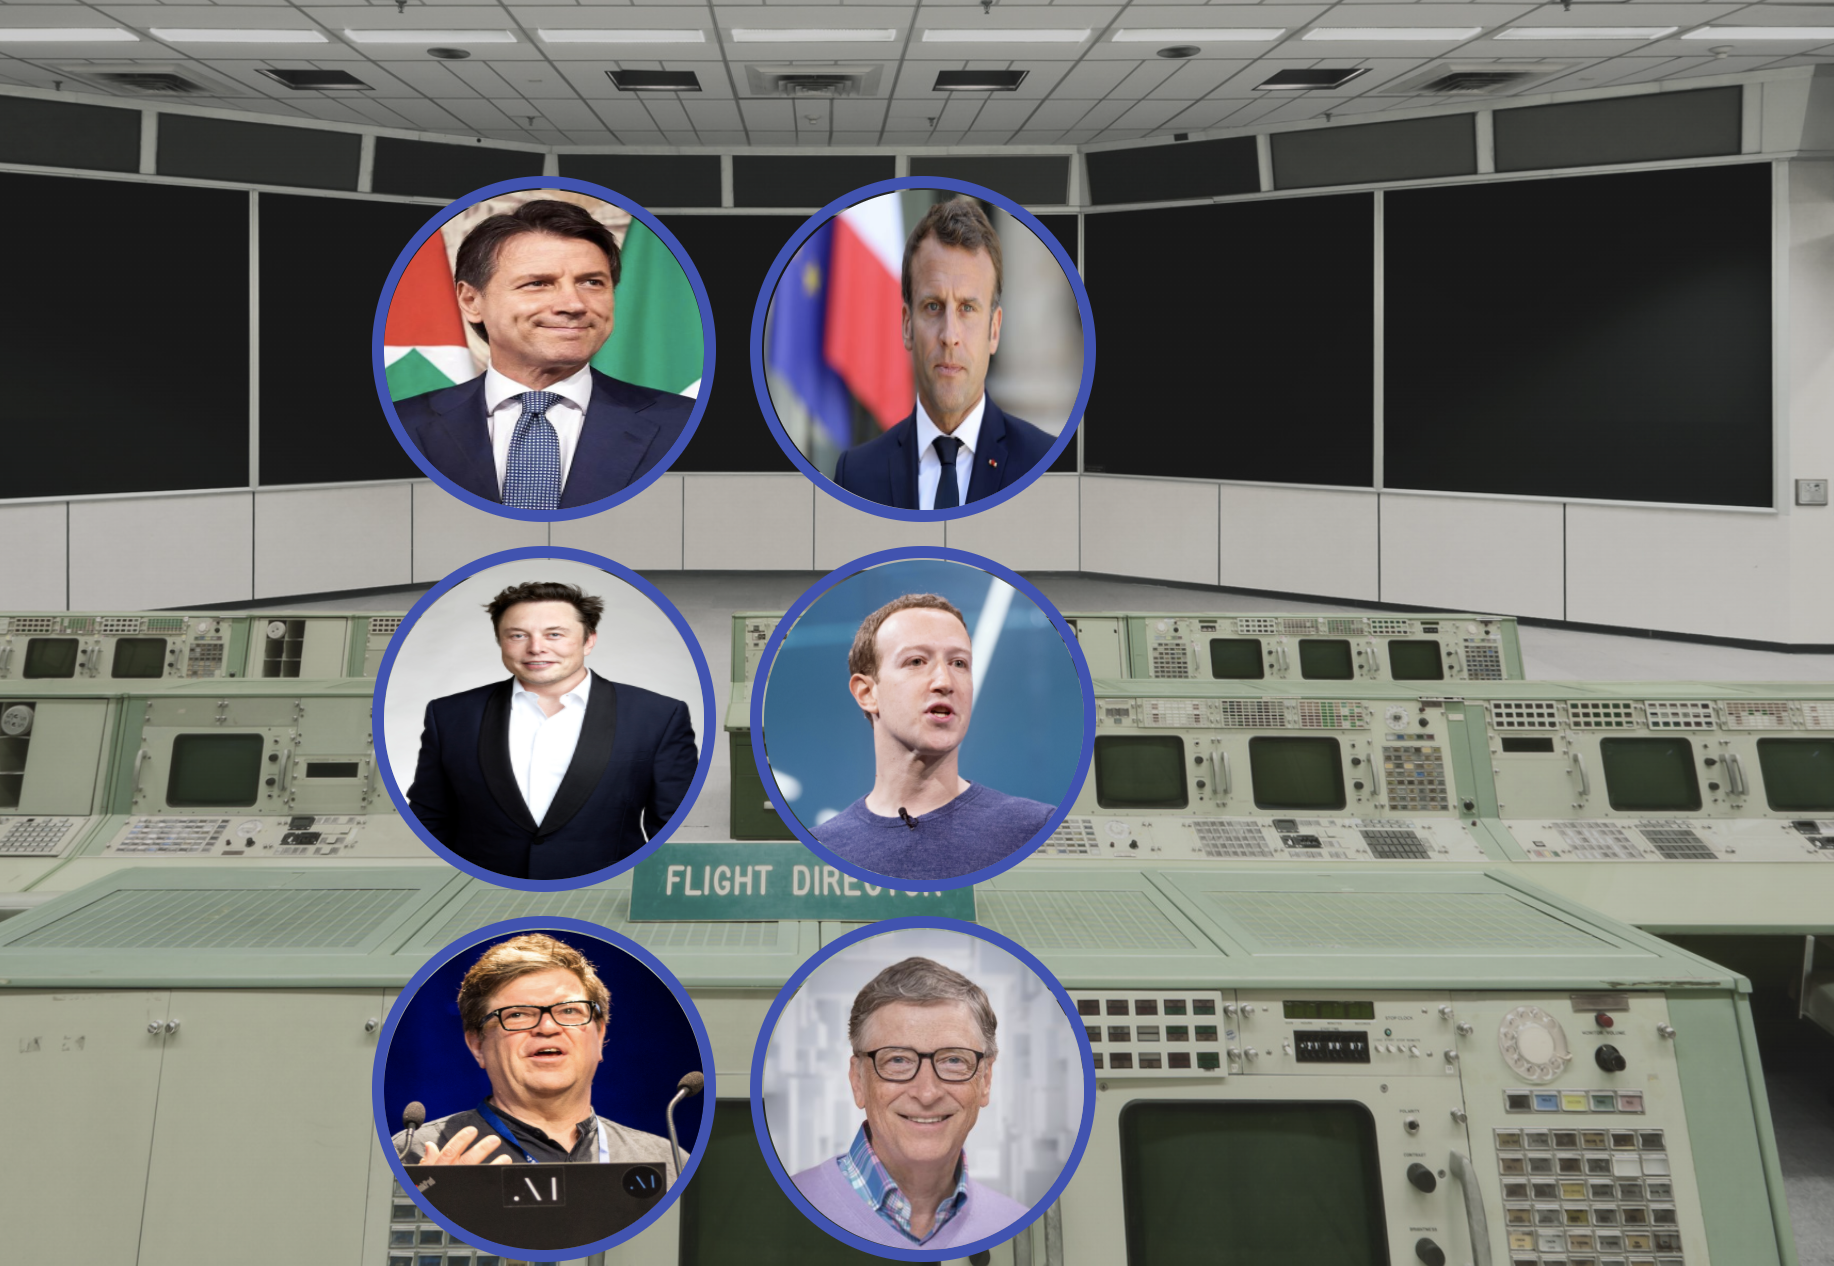
\includegraphics[width=16cm]{Resources/interface-intro.png}
  \caption{News Gathering Pipeline} 
\end{figure}

Once the user has been selected, you will enter the search screen that will allow you to make a query obtaining the results with respect to the tweets downloaded and used to generate the index.
By pressing on the customization switch and selecting a category you can get a customization of the search according to the user profile and the selected topic.

\begin{figure}[H]
  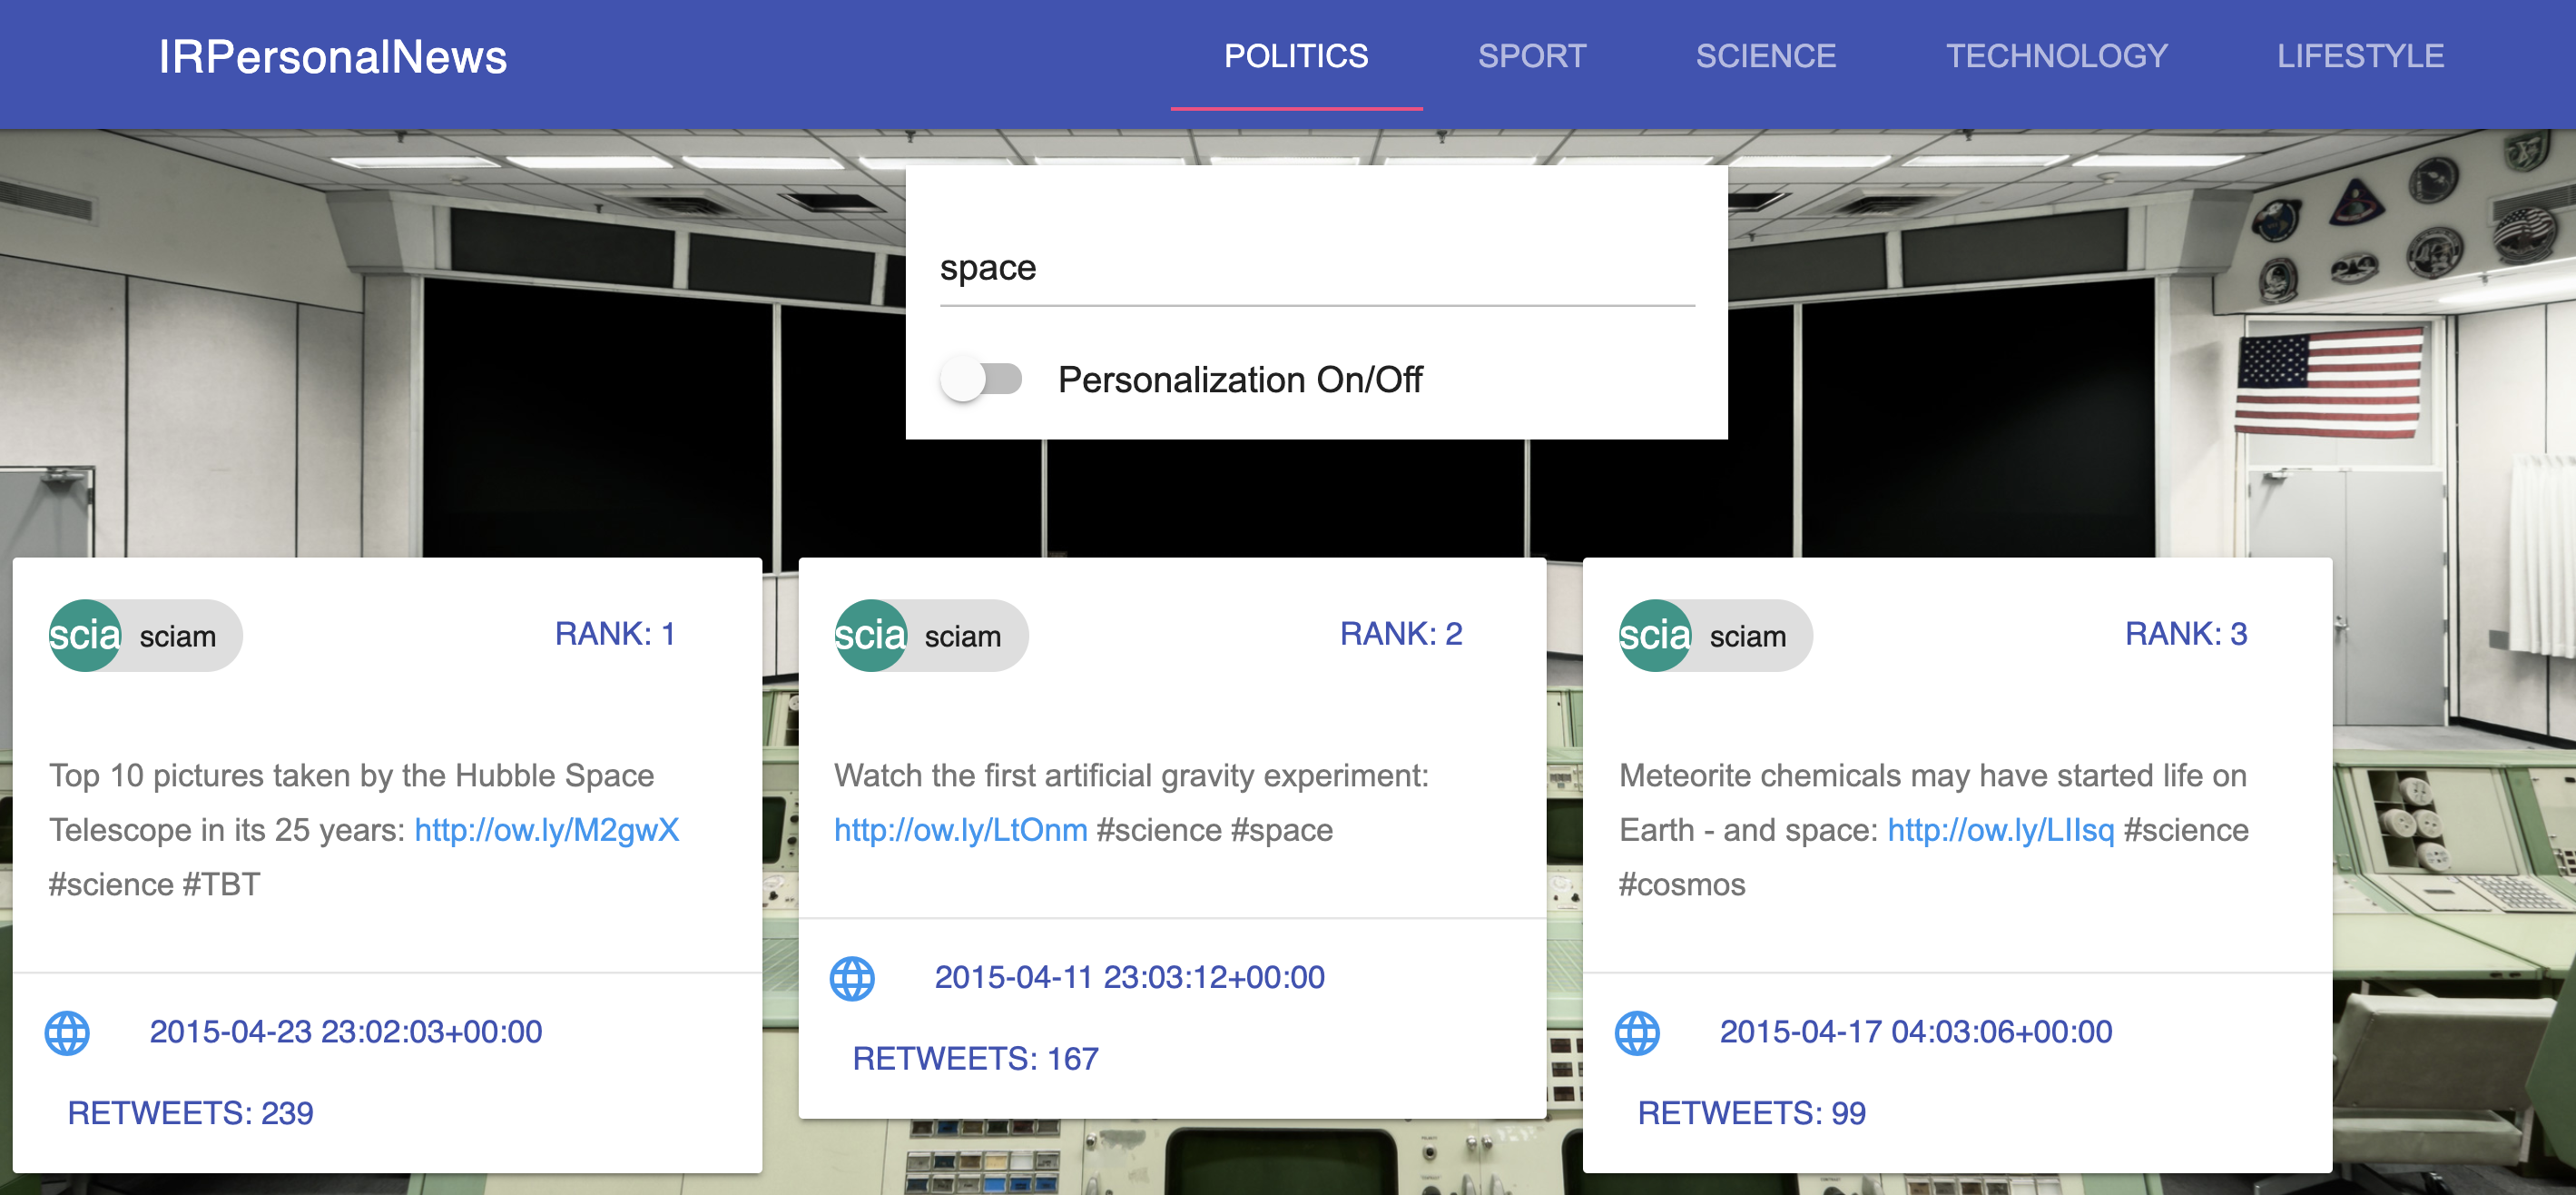
\includegraphics[width=16cm]{Resources/interface-search.png}
  \caption{News Gathering Pipeline} 
\end{figure}


\section{Conclusion and Future Work}

This project demonstrates how it is possible to create a system that allows to build a customizable search engine on users able to filter news from the web in an effective way.
\break
The purpose of this first version 1.0 is to demonstrate how the pipeline works.
\break
Certainly it is necessary to do more work to be able to put into production a stable and functioning application with these features, so as to modify the pipeline so that it is completely automatic and independent, both in obtaining information and in the creation of indexes and search.
\break
One feature that would certainly be of great help is to create custom user profiles directly on a web page, associating news from the web in the form of links.

\end{document}